\section{Coordinated Interaction}
\label{sec:foundations:mcv}

The interaction-design literature for analytical visualisation
converges on three reference points. Shneiderman's information-seeking
mantra (\textit{overview first, zoom and filter, details on
demand})~\cite{shneiderman1996eyes} sets the task-level architecture
the proposed system's Hub--Theme--Chart--Entity-Detail layering
follows. Yi, Kang, Stasko, and Jacko organise the interaction techniques
of information visualisation into seven user-intent categories: Select,
Explore, Reconfigure, Encode, Abstract/Elaborate, Filter, and
Connect~\cite{yi2007interaction}. Heer and Shneiderman group those
techniques into three umbrellas: data-and-view specification, view
manipulation, and process-and-provenance support, with twelve concrete
task types underneath~\cite{heer2012interactive}. Together the three
references establish that an interactive chart is not characterised by
its primitive (bar, scatter, heatmap) but by the set of user intents it
supports: a chart that allows no Select, no Filter, and no Connect is a
display widget rather than an analytical surface.

Within this space, the Multiple Coordinated Views (MCV) pattern is one
specific composition of the Yi categories. An MCV interface presents
the same dataset through several visualisations simultaneously and
propagates user interaction in one view to all of the others. The
defining property is coordination: selecting an entity in one chart,
whether by clicking a mark or by dragging a rectangular selection
across a region of the plot, causes the same entity to be highlighted
or filtered in every other chart on the same screen, so that the
analyst sees the same selection from multiple perspectives at
once~\cite{liu2022}. In Yi's terminology, MCV bundles Select with a
strong implementation of Connect that propagates across simultaneously
rendered sibling views.

The most common interaction primitive within MCV is brushing and
linking. Brushing is the act of selecting a subset of records in one
view, typically by dragging a rectangular brush over a region of the
plot or by clicking individual marks. Linking is the immediate
propagation of that selection to all coordinated views, so that the
brushed records are visually distinguished in every view in which they
appear. The combination is what gives MCV its analytical leverage: a
brush drawn across a range of one axis in a parallel-coordinates plot
becomes, in the linked map view, the highlighted spatial footprint of
the records that fall within that range, without any explicit query
having been written.

The model imposes design trade-offs. Coordinated propagation is
powerful but expensive: every view must re-render on every brush event,
which can degrade interactive latency on large datasets. The pattern
also presupposes that several sibling charts are visible on the screen
at the same time; user interfaces that render one chart per canvas
cannot expose simultaneous propagation to the reader. Scoping the
coordination locally, that is, restricting the propagation to a related
set of views that share an analytical theme rather than allowing it to
fan out across the entire interface, bounds both the cognitive load on
the user and the computational cost on the renderer. The analyst is not
forced to reason about how a selection in one corner of the interface
affects every other view, and the renderer does not have to refresh
charts whose relationship to the current selection would be incidental.

\begin{figure}[!htbp]
\centering
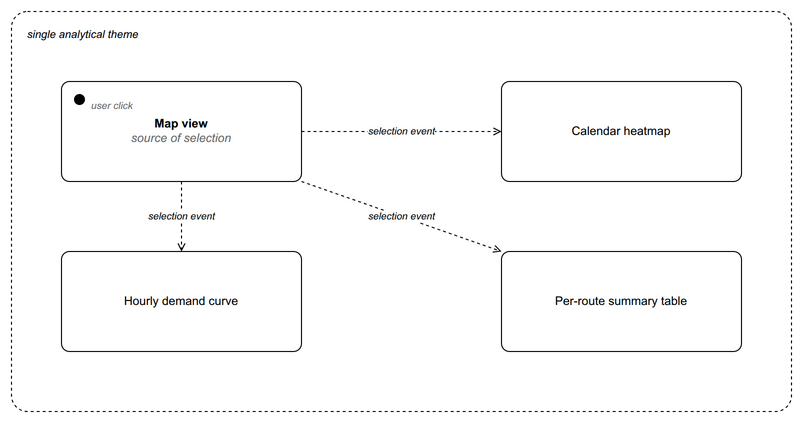
\includegraphics[width=0.92\linewidth]{images/diagrams/foundations_mcv.png}
\caption{Selection in one view propagating to coordinated views in the same theme.}
\label{fig:foundations:mcv}
\end{figure}

Section~\ref{sec:solution:interaction} selects from this design space.
It retains MCV as intellectual lineage and adopts the Yi (2007)
seven-category taxonomy as the criterion for chart inclusion (every
chart in the catalogue must support Select, Filter, and a Connect
realisation as a minimum). However, the proposed system implements
the Connect category not as simultaneous cross-chart propagation but as
a single click-to-entity-detail panel: clicking any entity in any
chart opens a side panel containing a multi-chart summary of that
entity. This realisation is consistent with the system's one-chart-per-canvas
shell, which would render MCV's simultaneous-brushing semantics
invisible to the reader, and is grounded in the Heer and
Shneiderman~\cite{heer2012interactive} observation that the
view-manipulation umbrella admits several Connect realisations of
different visibility and cost.
